\section{\textbf{Experimental Results}}
Our proposed suspicious text detection system is tested with logistic regression, naive Bayes, SVM,  KNN and decision tree classification algorithms. Table \ref{AE} represents accuracy and error rate of these algorithms on our dataset.
\renewcommand{\arraystretch}{1.5}
\begin{table}[h!]
\begin{center}
\caption{Evaluation Summary}
\begin{tabular}{||m{4.65cm} | m{1.4cm}| m{1.35cm}||}
\hline
     Classification Algorithm & Accuracy  & Error  \\
\hline
    Naive Bayes \cite{yoo2015classification} & 0.85 & 0.15\\
\hline 
    SVM (Linaer Kernel) \cite{wei2012text} & 0.91 & 0.09\\
\hline 
    SVM (RBF Kernel) \cite{villmann2017can}& 0.90 & 0.10\\
\hline 
    Logistic Regression\cite{sharma2015active} $_{proposed}$ & 0.92 & 0.08\\
\hline
    K-Nearest Neighbor \cite{harisinghaney2014text}& 0.73 & 0.27\\
\hline
    Decision Tree \cite{chavan2014survey}& 0.88 & 0.12\\
\hline
\end{tabular}
\label{AE}
\end{center}
\end{table}
\par
Table \ref{prr} shows the precision, recall and $F_1$ score of different classification algorithms used in our model.

\begin{table}[h!]
\begin{center}
\caption{Performance Comparison}
\begin{tabular}{||m{3.6cm} | m{1.25cm}| m{1.2cm}| m{1.3cm}||}
\hline
     Classification Algorithm & Precision & Recall & $F_1$ score \\
\hline
    Naive Bayes & 0.89 & 0.85 & 0.85\\
\hline 
    SVM (Linaer Kernel) & 0.91 & 0.91 & 0.91\\
\hline 
    SVM (RBF Kernel) & 0.90 & 0.91 & 0.90\\
\hline 
    Logistic Regression & 0.91 & 0.93 & 0.93\\
\hline
    K-Nearest Neighbor & 0.82 & 0.73 & 0.70\\
\hline
    Decision Tree & 0.88 & 0.92 & 0.89\\
\hline
\end{tabular}
\label{prr}
\end{center}
\end{table}

For all of the algorithms we used similar number of training and test documents. From table \ref{AE} and \ref{prr}, we can see that logistic regression and support vector machine algorithms are performing up to the mark on our dataset. Naive Bayes and decision tree also doing really well. But accuracy of K-nearest neighbour is really poor compared to other algorithms. 

Now, we will learn about classification report, precision-recall curve and receiver operating characteristic's (ROC) curve of this algorithms. Classification report gives us precision, recall and $F_1$ score of each category which is really helpful to analyze the algorithm
and find out shortcomings of the algorithms.
\par
\textbf{Table} \ref{NBC} to \textbf{Table} \ref{tdct} represents classification report and \textbf{Fig.} \ref{prrn} to \textbf{Fig.} \ref{fdct} shows precision-recall and ROC curve of all algorithms we used in our system.

\renewcommand{\arraystretch}{1.1}
\begin{table}[h!]
\begin{center}
\caption{Classification Report (Naive Bayes)}
\begin{tabular}{|m{2.8cm} | m{1.5cm}| m{1.3cm}| m{1.5cm}|}
\hline
     & Precision & Recall & $F_1$ score\\
\hline
     Suspicious & 1.00 & 0.71 & 0.83\\
\hline 
     Non suspicious  & 0.76 & 1.00 & 0.87\\
\hline 
     avg./total & 0.89 & 0.85 & 0.85\\
\hline
\end{tabular}
\label{NBC}
\end{center}
\end{table}

\begin{table}[h!]
\begin{center}
\caption{Classification Report (SVM Linear Kernel)}
\begin{tabular}{|m{2.8cm} | m{1.5cm}| m{1.3cm}| m{1.5cm}|}
\hline
     & Precision & Recall & $F_1$ score\\
\hline
     Suspicious & 0.91 & 1.00 & 0.91\\
\hline 
     Non suspicious  & 1.00 & 0.90 & 0.91\\
\hline 
     avg./total & 0.91 & 0.91 & 0.91\\
\hline
\end{tabular}
\label{SVML}
\end{center}
\end{table}

\begin{table}[h!]
\begin{center}
\caption{Classification Report (SVM RBF Kernel)}
\begin{tabular}{|m{2.8cm} | m{1.5cm}| m{1.3cm}| m{1.5cm}|}
\hline
     & Precision & Recall & $F_1$ score\\
\hline
     Suspicious & 0.90 & 0.99 & 0.90\\
\hline 
     Non suspicious  & 0.99 & 0.89 & 0.91\\
\hline 
     avg./total & 0.90 & 0.91 & 0.90\\
\hline
\end{tabular}
\label{SVMR}
\end{center}
\end{table}

\begin{table}[h!]
\begin{center}
\caption{Classification Report (Logistic Regression)}
\begin{tabular}{|m{2.8cm} | m{1.5cm}| m{1.3cm}| m{1.5cm}|}
\hline
     & Precision & Recall & $F_1$ score\\
\hline
     Suspicious & 0.92 & 1.00 & 0.93\\
\hline 
     Non suspicious  & 1.00 & 0.93 & 0.93\\
\hline 
     avg./total & 0.91 & 0.93 & 0.93\\
\hline
\end{tabular}
\label{lr}
\end{center}
\end{table}

\begin{table}[h!]
\begin{center}
\caption{Classification Report (K-Nearest Neighbor)}
\begin{tabular}{|m{2.8cm} | m{1.5cm}| m{1.3cm}| m{1.5cm}|}
\hline
     & Precision & Recall & $F_1$ score\\
\hline
     Suspicious & 0.65 & 1.00 & 0.79\\
\hline 
     Non suspicious  & 1.00 & 0.44 & 0.61\\
\hline 
     avg./total & 0.82 & 0.73 & 0.70\\
\hline
\end{tabular}
\label{tknn}
\end{center}
\end{table}

\begin{table}[h!]
\begin{center}
\caption{Classification Report (Decision Tree)}
\begin{tabular}{|m{2.8cm} | m{1.5cm}| m{1.3cm}| m{1.5cm}|}
\hline
     & Precision & Recall & $F_1$ score\\
\hline
     Suspicious & 0.91 & 0.89 & 0.90\\
\hline 
     Non suspicious  & 0.88 & 0.90 & 0.89\\
\hline 
     avg./total & 0.90 & 0.90 & 0.90\\
\hline
\end{tabular}
\label{tdct}
\end{center}
\end{table}

\begin{figure}[H]
\centering
\subcaptionbox{precision-recall}{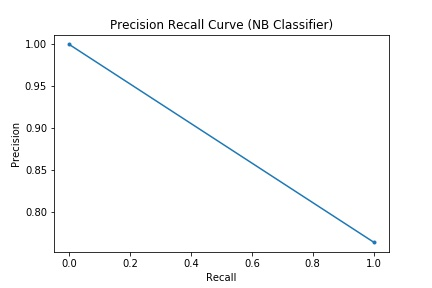
\includegraphics[scale=0.29]{Figures/PRN.jpg}}%
\hfill % <-- Seperation
\subcaptionbox{ROC}{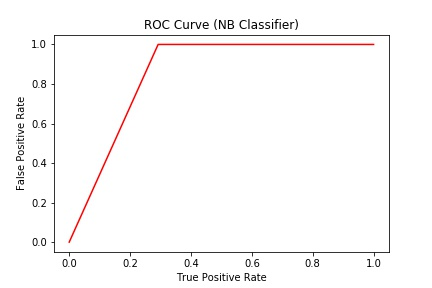
\includegraphics[scale =0.29]{Figures/ROCN.jpg}}%
\caption{Result of Naive Bayes Classifier}
\label{prrn}
\end{figure}

\begin{figure}[H]
\centering
\subcaptionbox{precision-recall}{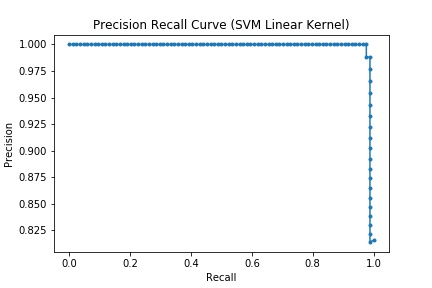
\includegraphics[scale=0.29]{Figures/PRSL.jpg}}%
\hfill % <-- Seperation
\subcaptionbox{ROC}{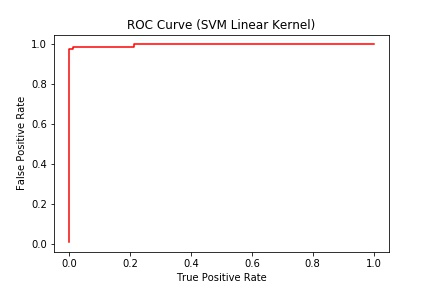
\includegraphics[scale =0.29]{Figures/ROCSL.jpg}}%
\caption{Result of SVM (Linear Kernel)}
\label{slk}
\end{figure}

\begin{figure}[H]
\centering
\subcaptionbox{precision-recall}{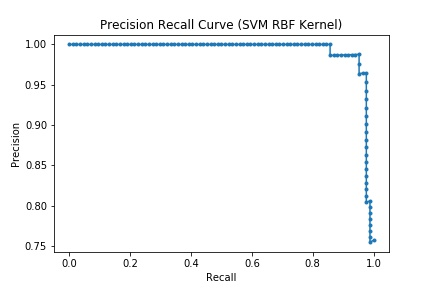
\includegraphics[scale=0.29]{Figures/PRSR.jpg}}%
\hfill % <-- Seperation
\subcaptionbox{ROC}{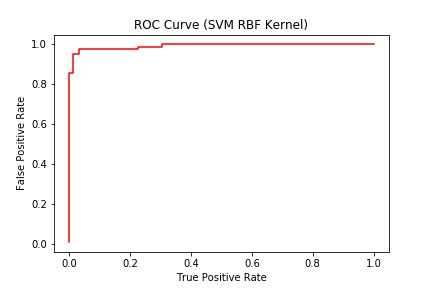
\includegraphics[scale =0.29]{Figures/ROCSR.jpg}}%
\caption{Result of SVM (RBF Kernel)}
\label{svr}
\end{figure}

\begin{figure}[H]
\centering
\subcaptionbox{precision-recall}{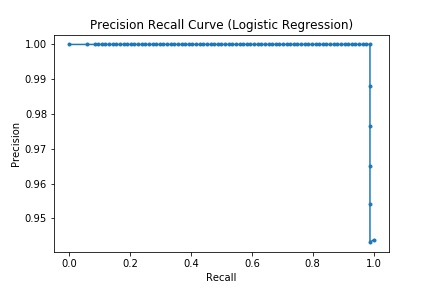
\includegraphics[scale=0.29]{Figures/PRLR.jpg}}%
\hfill % <-- Seperation
\subcaptionbox{ROC}{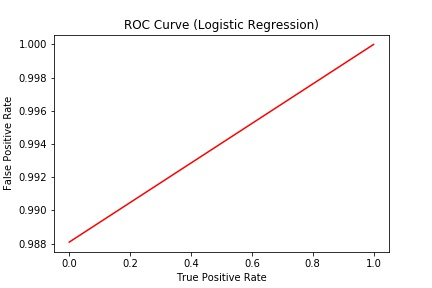
\includegraphics[scale =0.29]{Figures/ROCLR.jpg}}%
\caption{Result of Logistic Regression}
\label{flr}
\end{figure}

\begin{figure}[H]
\centering
\subcaptionbox{precision-recall}{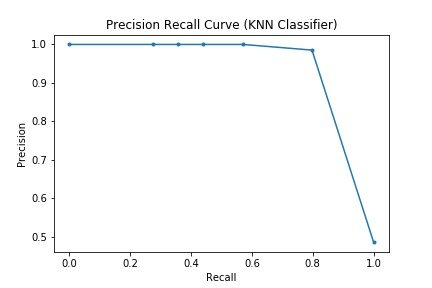
\includegraphics[scale=0.29]{Figures/PRKNN.jpg}}%
\hfill % <-- Seperation
\subcaptionbox{ROC}{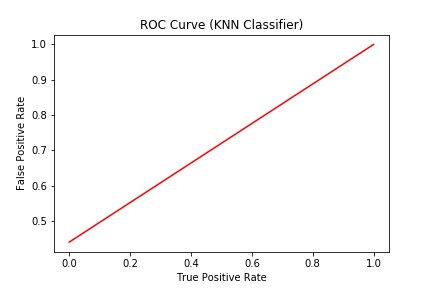
\includegraphics[scale =0.29]{Figures/ROCKNN.jpg}}%
\caption{Result of K-Nearest Neighbor}
\label{fknn}
\end{figure}

\begin{figure}[H]
\centering
\subcaptionbox{precision-recall}{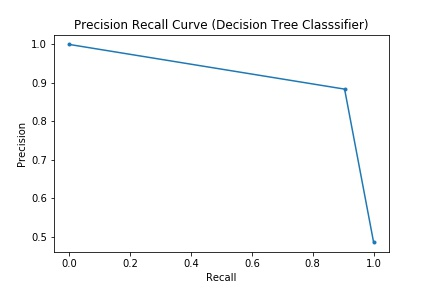
\includegraphics[scale=0.29]{Figures/PRDCT.jpg}}%
\hfill % <-- Seperation
\subcaptionbox{ROC}{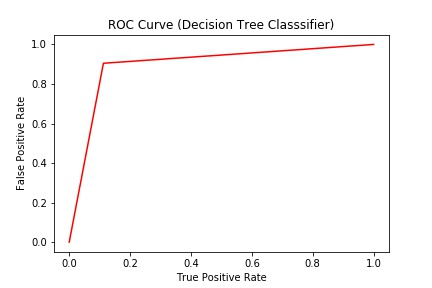
\includegraphics[scale =0.29]{Figures/ROCDCT.jpg}}%
\caption{Result of Decision Tree}
\label{fdct}
\end{figure}

\textbf{Fig.} \ref{fig:out} shows sample input and corresponding output in our system.
\begin{figure}[h!]
\centering
  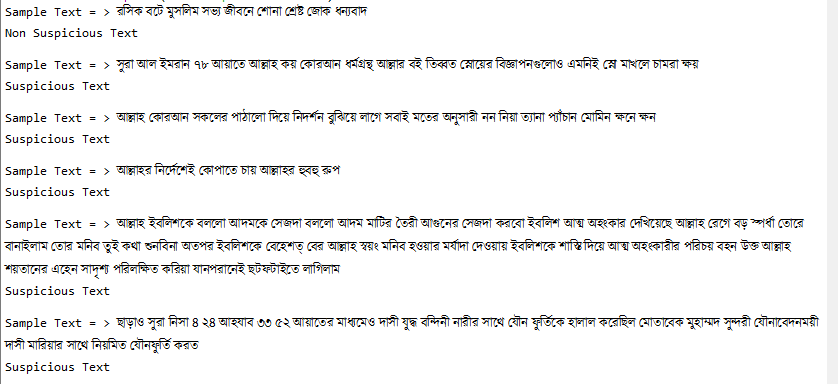
\includegraphics[height=6.8cm, width=8.8cm]{Figures/output.PNG}
  \caption{ Output in System Environment}
  \label{fig:out}
\end{figure}